\chapter{Background}

% SIDDATA (mit Educational Resources dabei, muss kein sub-chapter sein)
% Conceptual Spaces (What is this?)
% Required techniques and algorithms

\section{Replication and Software Quality}

\includeMD{pandoc_generated_latex/2_0_replication}

\section{SIDDATA and Educational Resources}

\includeMD{pandoc_generated_latex/2_0_siddata}

\section{Conceptual Spaces}

This section will introduce conceptual spaces as tool of choice as well as how to generate them and how reasoning on them works, as well as some other related work to what's done in this thesis.

\subsection*{Theory of Conceptual Spaces}

The theory of Conceptual Spaces was first introduced by Peter Gärdenfors in his 2000 book \citetitle{Gardenfors2000a} \cite{Gardenfors2000a} both as a theoretical model of human concept formation, but also as format for knowledge representation in artificial systems \cite{Gardenfors2004}. 

On the one hand, \glspl{cs} should serve as bridge between symbolistic and connectionistic approaches to knowledge representation. By having CS as layer of reasoning and representation in between both, classical symbols would be grounded in noisy high-dimensional data, allowing for high-level syllogistic reasoning from real-world data. 

If a computer has a knowledge base that says $\exists x.Red(x) \& Apple(x)$, does it know what "red" and "apple" mean? We need to ground symbols, to express meaning!

According to Gärdenfors, concept-representation in humans is represented by three levels of accounting for observations: The symbolic level, the conceptual level and the subconceptual level \cite[204]{Gardenfors2000a}:
\begin{description}
    \item[Subconceptual] Observations are the firing of the neurons of our sensory receptors, without any conceptualization.  (connectionism, \glspl{ann})
    \item[Conceptual] Observations are defined not as token of a symbol, but as vector in a conceptual space of some quality  (prototype theory, linear algebra)
    \item[Symbolic] represents observations by describing them in some specified language (formal logic, syllogisms, symbolism, classical AI, logical positivism)
\end{description}

Importantly, these levels are not in conflict, but different models of the same phenonemon where each cover distinct important aspects. The process of inducing a general rule from few samples for example is represented as pattern-matching on the firing patterns in the subconceptual level, which translates to the conceptual level as geometric reasoning through regions and direction. As another example, semantic relations such as hyponyms from the symbolic level are modelled as geometric sub-regions on the conceptual level. So on the one hand, automatically generated conceptual spaces could allow for high-level syllogistic reasoning on real-world data without the need to manually add countless facts. However it also provides a new way to model reasoning and inference for both other levels through geometric relations, providing explanations for the noisy subconceptual level and computationally less complex algorithms for the symbolic level. The validity of the statement \textit{a robin is a bird} is given because robins are gemmetrically a subregion of the region of birds.

So on the one hand it's a framework for scientific theories, but on the other hand a model of human concept formation from phenomenal observations. Regardless of the theory's aspiration to accurately model human conceptualization and reasoning, it provides a useful knowledge representation method and tool that allows to model kinds of human reasoning with novel algorithms that cannot be done with both other well-researched methods \cite[Sec.~6.7]{Gardenfors2000a}. 

In practical applications, it can serve as representational format to express semantic relations for the semantic web \cite{Gardenfors2004}. After years of trying to model information processing through pure deductive reasoning and classical ontologies (\eg RDS, OWL or WordNet), turns out there may be be more to it than strict is-a relationships and explicit, unambiguous, universal truths, as for example similarity, which CS can model due to its richer semantic structure. 

\subsection*{Definition}

\todoparagraph{iff = if and only if}

In conceptual spaces, concepts are represented as convex regions in domain-specific, human-interpretable spaces. For example, the concept of "apple" is a region that in the dimension "color" is somewhere between red and green, in the dimension "form" at roughly round, in the dimension "taste" somwhere between sweet and sour, etc. Every instance of an apple is thus a vector that lies inside the region of the concept. This allows for high-level reasoning, such as the question "does any Instance of concept X fit into my bag?" -> If the "size" dimension of the whole region is smaller than the size of my bag, it will.

\begin{figure}[H]
	\centering
	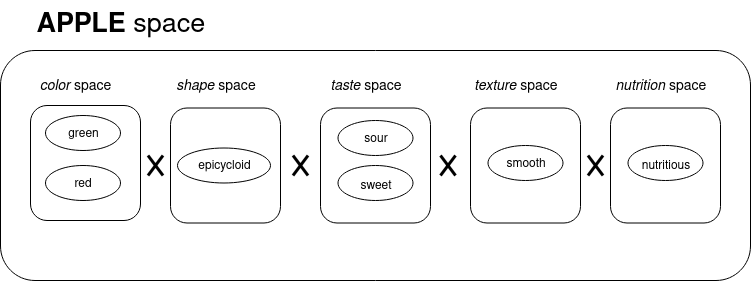
\includegraphics[width=\textwidth]{graphics/stolenfigures/apple_space.png}
	\slcaption{
		CS for an apple. Stolen from \cite{Hernandez-Conde2017}, who in turn stole it from xyz
	}
\end{figure}



\fbox{\begin{minipage}{37em}
    \newtheorem*{theorem*}{Conceptual Space}
    \begin{theorem*}
        A conceptual space is a geometric structure used to encode the meaning of natural language terms, properties and concepts. The metric space is spanned by \emph{quality dimensions} denoting basic domain-specific properties based on perception or sub-symbolic processing. Natural language categories (\emph{concepts}) correspond to convex regions, whereas points denote individual objects (instances/\emph{entities}, allowing for geometric solutions to commonsense reasoning tasks such as \emph{betweeness} or \emph{induction}.
        % \cite{Derrac2015}: "Conceptual spaces \cite{Gardenfors2000a} are metric spaces which are used to encode the meaning of natural language concepts and properties."
    \end{theorem*}
\end{minipage}}

Formally defined, a conceputal spaces needs the following definitions:
\begin{description}
    \item[Quality Dimensions] are atomic units of perception. Some of these are necessarily linked (such as hue and saturation), making them \textit{integral}, whereas others (\eg. temperature and weight) are \textit{seperable}. Typically each dimension corresponds to a primitive cognitive feature.
    \item[Domain] A set of integral dimensions that are seperable from others, like the \textit{color} domain made up from hue, saturation and value. Conceptual spaces are grouped into several low-dimensional subspaces according to these domains.
    \item[Similarity] is defined as inverse distance, which requries a metric. A distinction can be made for the aggregation of integral and separable dimensions. 
    \item[Betweenness] An object Y is between two other objects X and Z iff d(x,y) + d(y,z) = d(x,z).
    \item[Natural Properties (\textit{criterion P} \cite{Gardenfors2000a})] are defined as convex regions of a domain in a conceptual space. A convex region has the property that an interpolation between any two points in this region is necessarily also in this region. 
    \item[Concepts (\textit{criterion C} \cite{Gardenfors2000a})] are combinations of (potentially correlated) properties. \q{A concept is represented as a set of convex regions in a number of
    domains together with a prominence assignment to the domains and information about how the regions in different domains are correlated} \cite[8]{Gardenfors2004}
    \item[Entities] are specific instances (tokens) of a concept, encoded as points. 
    \item[Context] can be modelled in a CS by weighting certain dimensions higher than others, influencing distance and how concepts are fromed from properties.
\end{description}

Some corollaries: 

\begin{itemize}
    \item Each conceptual space contains only items for which the space's dimensions make sense, so you wouldn't find kings in a conceptual space of cabbages.
    \item Concepts roughly correspond to (non-proper) nouns, adjectives to properties and proper nouns (the name of a particular person, place, organization, or thing to points.)
    \item Concept combination depends on the compatibility of the respective domain: For fully compatible domains, this narrows the new concept down (a \textit{green banana} is both green and bitter). If the modifier is incompatible with the original vaue, it replaces that information (\eg a \textit{pink elephant}), furhter replacing other incompatible domains (\eg to a \textit{stone lion}, the concepts of \textit{habitat} and \textit{life span} don't apply).
    \item From the criterion of convexity for natural properties and the definition of betweenness, it follows that if an object Y is between X and Z, and both X and Z have a property, Y must also have this property.
    \item Relative properties can be defined as regions on a relative scale - the property "\textit{tall}" acccordingly can be defined to be true iff the entity is in the top 33\% \wrt the size-property of all relevant objects.
\end{itemize}

% \includeMD{pandoc_generated_latex/2_2_conceptualspaces}
\todoparagraph{look if I want to take a paragraph from 22conceptualspacesMD}
\todoparagraph{Rudiger had a formal definition in the CS course}

\subsection{Data-Driven Generation of Conceptual Spaces}

\includeMD{pandoc_generated_latex/2_3_datadrivengeneration}

\subsection{Explainable Reasoning with Conceptual Spaces}
% was "computational reasoning"
\label{sec:reasoning}

\todoparagraph{important for us is that we} don't have ONE SINGLE SIMILARTIY; BUT THAT IT's context-dependent!!!!

\todoparagraph{However a short paragraph about reasoning-based classifiers and the respective intutitive explanations for known classifiers}

The goal of this thesis is to provide explainable recommendation for educational resources. This section elaborates how the framework of \glspl{cs} allows to computationally model commonsense reasoning through analytic geometry and algebra.

\todoparagraph{We are looking how symbolistic stuff relates to CS}

According to \cite{Gardenfors2000a}, Representations don't need to be similiar to the objects they represent, but the *similarity relations of the representations* should correspond to those of the objects they represent

\subsubsection*{Categories and Ontologies}

% CS and with it ontologies "automatically" (BIG question mark) arise from prototypes + metric domain + voronoi tesselation

\todoparagraph{Vor allem sollte hier ruberkommen warum das gut fur mich und meinen recommender fur educational resources ist argh}

Logic-Based reasoning/inference can do many things already, however it requires the knowledge to be encoded in logic (a lot of manual work) and doesn't allow for fuzzyness.
In formal logic/ontologies/lexical databases, semantic relations of concepts are explicitly modelled. The \gls{rcc} \cite{Cohn1997a} links these relations to their geometric interpretation, providing a bridge between this and Conceptual Spaces \cite{Gardenfors2001}. Once you have created the structure, the following emerges automatically:

\vspace{2ex}

\begin{tabularx}{1.05\textwidth}{P{0.16\textwidth}|P{0.25\textwidth}|P{0.25\textwidth}|X}
    Ontology Relation & Other Names        & RCC5 \cite{Cohn1997a} analog / \textit{Geometric equivalent} & Example \\ \midrule

    Type Identity     & {\scriptsize Equality of Concepts, Synonymy } & Identical Regions (EQ)      & Animals with a liver \& Animals with a heart \\ 

    Subsumption       & {\scriptsize Hyponyms/ Hypernyms, \textit{is-a-relationship}, Concept Hierachies, Taxonomies }
                                           & Proper Parts(PP, PP\textsuperscript{-1}), \textit{Subregions}
                                                                          & \textit{Every pizzaria is a restaurant} \\  
    
    Mutual 
    Exclusiveness     &                    & Discrete Regions (DR), \textit{unconnected/disjoint regions}
                                                                          & \textit{No Restaurant can be a beach} \\  

    Overlapping 
    Concepts          &                    & Partial Overlap (PO)         & \textit{Some bars serve wine, but not all} \\  

    Opposites         &                    & \textit{Set inverse}         & Humans \& Non-human animals \\ 

    Token Identity    & {\scriptsize Equality of Names, Synonymy } & \textit{Equal coordinates}   & Morning star \& Venus \\ 
    Meronymy / Holonymy & {\scriptsize \textit{part-whole realationship} }& -             & Trees \& Leaves
\end{tabularx}

\vspace{4ex}

% Also: characteristics of properties (transitivity, symmetry) (from intrinsic features of dimensions (time is linear because the dimension is linear))

So for example the validity of "a robin is a bird" is encoded by it being a subregion. So, no reason for a symbolic inference when using the richer structure of CS instead of ontologies.

So except Meronymy, a CS can model all semantic relations of classical ontologies/formal logic/symbolistic approaches/knowledge bases. However as it encodes more than just a taxonomy of concepts, it for higher/more forms of inference and (common-sense) reasoning, among others by enabling for interpolation and extrapolation of knowledge. These are:

\subsubsection*{Similarity-based reasoning}

\label{sec:similaritybasedreasoning}

As discussed already in \autoref{sec:amazonalgo}, modern recommendation algorithms often rely on similarity-based reasoning by suggesting that users that liked and item may also like similar items (collaborative filtering). In terms of classification, this corresponds to the 1-Neirest-Neighbor approach, where an object is assigned the class of the most similar item:\footnote{1-NN: \textit{Y is of the same class as X because X closest to Y}}

\noindent
\begin{minipage}{.6\textwidth}
  \syllogism{Alice likes \textit{the Lord of the Rings} \\
           \textit{The Hobbit} and \textit{Lord of the Rings} are similar}{Alice will probably like \textit{The Hobbit}}
\end{minipage}% 
\begin{minipage}{.4\textwidth}
  \syllogism{\textbf{A} has property \textbf{x} \\
             \textbf{B} is  similar to \textbf{A}}
             {\textbf{B} likely also has property \textbf{x}}
\end{minipage}% 

\vspace{2ex}

This is something that cannot be done by classical logic, which can not model degrees of something but only universal full truths. Another advantage is that it's easy to train, however a disadvantage is that it requires enough similar concepts which may not be given This algorithm however lacks \textit{explainability}: The employed distance function does not encode \textit{in what respect} two items are similar. For human reasoning however, there is no \textbf{overall Similarity} - instead similarity is relative to a domain and only meaningful in context \cite{Goodman1972-GOOPAP-3}: \q{any measurement of similarity is based on assumptions concerning the properties of a similarity relation} \cite[110]{Gardenfors2000a}. In a conceptual space, this can be modelled: The distance function can give weight for certain dimensions depending on context or objects of different concepts can be considered similar if they share enough properties. Most importantly however, in a CS a system for recommendation can ask users what dimensions of a given entity the user liked to suggest items that are similar in that regard.
% a system serving me a similar wine to the one I want that is not available can ask me what dimensions of that wine were important before suggesting new ones.

\subsubsection*{Induction}

Another very important tool of human common-sense reasoning is abstraction/generalization/ \textbf{induction}, going from single observations to general rules. For that, we need to decide which properties of the respective observation are relevant, distilling sensible information from the receptors from unimportant information to make inferences from limited information about an object? The connectionistic answer to that would be "pattern matching", and ML algorithms work extremely well for that, however this lacks explainability, and also we want to model the underlying algorithm and the underlying patterns. All three levels can model some kinds of induction and generalization, remember they are not in conflict. On the Conceptual Level you can eg model \textit{If two different entities of the same class have a property, maybe all entities of that class have a property}, which would be \textit{categroical inductive inverences}

\syllogism{Grizzly bears love onions \\
Polar bears love onions}
{All bears love onions \cite[226]{Gardenfors2000a}}

Other kinds of inductive reasoning we can model:

\textbf{Interpolative Reasoning}

\cite{Schockaert2011}: \q{intermediary conditions lead to intermediary conclusions} 

\noindent
\begin{minipage}{.6\textwidth}
  \syllogism{Cars have tires \\
             Bikes have tires \\
             Motorcycles are between cars and bikes
             }{Motorcycles likely also have tires}
\end{minipage}% 
\begin{minipage}{.4\textwidth}
    \syllogism{\textbf{A} has property \textbf{x} \\
               \textbf{C} has property \textbf{x} \\
               \textbf{B} is conceptually between \textbf{A} and \textbf{C}}
               {\textbf{B} likely also has property \textbf{x}}
\end{minipage}% 

% Source looking into it ([28] of [DESC15]): M. Abraham, D. Gabbay, U. Schild, Analysis of the talmudic argumen- tum a fortiori inference rule (kal vachomer) using matrix abduction, Studia Logica 92 (2009) 281–364.

\vspace{2ex}
\textbf{A fortiori reasoning}

\noindent
\begin{minipage}{.6\textwidth}
    \syllogism{\textit{The shining} is a horror film \\
            \textit{The shining} is scary \\
            \textit{It} is more scary than \textit{The shining}}
            {\phantom{penis} \\ 
            \textit{It} is likely also a horror film}
\end{minipage}% 
\begin{minipage}{.4\textwidth}
    \syllogism{\textbf{A} has property \textbf{x} \\
               \textbf{B} is \textit{more severe} than \textbf{A} \\ \phantom{penis}}
               {\textbf{B} likely also has property \textbf{x} \\ 
               \vspace{-0.5em} or a \textit{more severe} property}
\end{minipage}% 

\vspace{2ex}

\textbf{Extrapolative reasoning (Analogical Reasoning)} \cite{Schockaert2011}: \q{Analogous changes in the conditions should lead to analogous changes in the conclusion}, or \q{Concepts which differ in analogous ways have properties which differ in analaogous ways}. This is \textit{relational similarity}: If the analogical proportion a : b :: c : d holds, the pairs (a, b) and (c, d) are called relationally similar. Simply maps to geometric parallelism. 

I wrote down the syllogisms here, however that's not the only way to apply it, I can also "look for things that". In the case of analogies, I can ask "what is the thing that behaves to waterski like snowboarding to skiing"?

\textbf{Metaphors / Metonymy} (saying "the Pentagon" when referring to the US military) follow from a fortiori/analogical reasoning


\begin{figure}[H]
	\centering
	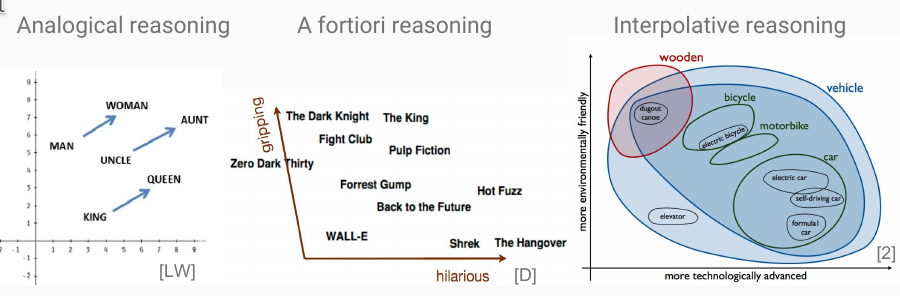
\includegraphics[width=\textwidth]{graphics/stolenfigures/reasoning_samples.png}
	\slcaption{
		Different forms of reasoning represented graphically. Holy shit remove me
	}
    \label{fig:graphic_reasoning}
\end{figure}

To automate these forms of inference, we need a richer form of knowledge than what is available in calssical logic: We need a notion of / Information about \textbf{Betweenness} and \textbf{Directionality}.

To model the stuff in \autocite{fig:graphic_reasoning}, we need a good metric, and what we see there definitely sounds euclidian!

\textbf{Summarized, CS are better than symbolism because we save the inference engine (plus we can extend and simulate knowledge bases with commonsense reasoning, just like humans deal with incomplete knowledge!) and better than connectionism because they are explainable. Klar soweit?!}

\todoparagraph{The problems of polysemy und synonymy for classical stuff, see fundamental information retrieval problem}


% \includeMD{pandoc_generated_latex/2_4_typesofreasoning}

\section{Other Related Work}
\label{sec:otherwork}

This thesis will focus on the aforementioned algorithm, primarily considering \cite{Derrac2015} and on top of that only two follow-up works: \cite{Ager2018, Alshaikh2020}, which have shown to provide useful extensions for it without changing its core logic. This shall by no means mean that these are the only ones that could be considered.

\paragraph{Tag Genome} 

By far the closest to what we do is the algorithm of \textcite{VISR12}, who generate a so-called tag genome for the domain of movies supervisedly based on keywords that users have assigned manually. Their algorithm takes these binary assignments and creates a dense representation that encodes a degree of relevance for each combination of movie and tag. Furthermore, they create a dedicated movie recommendation system on basis of this (interface reprinted in \autoref{fig:movietuner}). This system provides explainable recommendation based on these tags, allowing users to request recommendations for movies such as \textit{\q{I‘d like something less violent than Reservoir Dogs}} \cite[3]{VISR12}. Not only is their application exactly what is being demanded here, but the algorithm itself also performed significantly better than the one of \textcite{Derrac2015} in a human study of the latter, in which they directly compared the techniques by asking subjects which of the respectively extracted keywords better describes the difference between two movies \cite[44]{Derrac2015}. Considering however that \gencite{VISR12} algorithm is supervised and requires data which does not exist for our domain, it cannot be applied in our case. On the contrary, the final results of their algorithm are preferred by users over the ones generated with the algorithm considered in this work, but structurally exactly equal. This provides clear evidence that the desired application of this work is possible, albeit of lower quality than what their work achieved.

Generally, what is being done here corresponds to \textbf{Representation Learning}, whose aim is to discover the inherent semantic structure of a representation unsupervisedly \cite{Dayan1995}. More specifically \textbf{Disentangled Representation Learning}, where only salient attributes relevant to the task at hand should be extracted, which means finding latent embeddings whose dimensions are meaningful interpretable features. Generative Adversarial Networks \cite{Goodfellow2014} or Variational Autoencoders \cite{Kingma2013} are modern techniques that are good at finding latent information in images. Especially InfoGAN \cite{Chen2016} should be named, which can extract interpretable features such as pose, hairstyle, prensence of glasses and emotions from images unsupervisedly. 


\paragraph{LDA} 
\label{sec:lda}

In the realm of \gls{nlp}, this also relates to \textbf{Topic Modeling}, which aims to extract multiple hidden themes from a given text corpus by discovering groups of co-occuring words unsupervisedly. A well-known algorithm for this is Latent Dirichlet Allocation (LDA) \cite{Blei2003}, which represents documents by its salient \textit{topics}, each of which being a cluster of natural language terms. This technique bases on the assumption that each text consists of various topics, which are in turn made up by various keywords, making it possible to represent texts as multinomial distribution over latent topics which are aggregations of these keywords. Assuming a hierachical bayesian distribution where each text of a corpus is represented as mixture of topics it contains, their unsupervised algorithm extracts these by approximating the underlying infinite mixture of topic with an expectation-maximization (EM) algorithm. This yields a representation where each text is explicitly represented by the most propable words according to this distribution for a finite number of most probable topics. The algorithm finds use in text classification and collaborative filtering, but relies on unflexible \gls{bow} representations, making it hard to incorporate additional information such as correlations between topics \cite{Ager2018}.


\paragraph{Academic Interests Recommender}

Regarding the used domain, there is already a system incorporated into the Siddata-\gls{dsa} that aids students by finding and recommending educational resources. SidBERT \cite{Schrumpf2021DELPHI} extracts implicit information from courses and other learning material by their title by categorizing them into one of 905 classes derived from the third or fourth level of the \gls{ddc} \cite{Dewey1876}, a hierachical tree stucture system commonly used to categorize library books. SidBERT uses the same dataset as this work and classifies with a custom classification head ontop of a \gls{bert}-encoder \gls{ann} which is trained on 1.3 million book titles collected from three universities as well as the German National Library, currently achieving 45.2\% test accuracy (62.2\% recall) among 905 classes.

\includeMD{pandoc_generated_latex/2_5_relatedwork}


\section{Relevant Algorithms and Techniques}
\label{sec:required_algos}

\todoparagraph{dont forget the links for lsa und lda - are in lsa-long-md }

Thus far, we have described the base algorithm that this thesis replicates. Before describing each of its step in details, it is useful to get a grasp of some general concepts of its components. Furthermore, we will to put it into the context of the field of computational \gls{nlp} and some of the required theoretical foundation and quickly look at what other tools can be used for some of its components.


















\includeMD{pandoc_generated_latex/2_7_seperatrixdistance}

\includeMD{pandoc_generated_latex/algo_problems.md}
